\tikzset{%
    every neuron/.style={
        circle,
        draw,
        minimum size=5pt,
        inner sep=0pt,
        very thin
    },
    neuron/.style={
        fill
    },
}

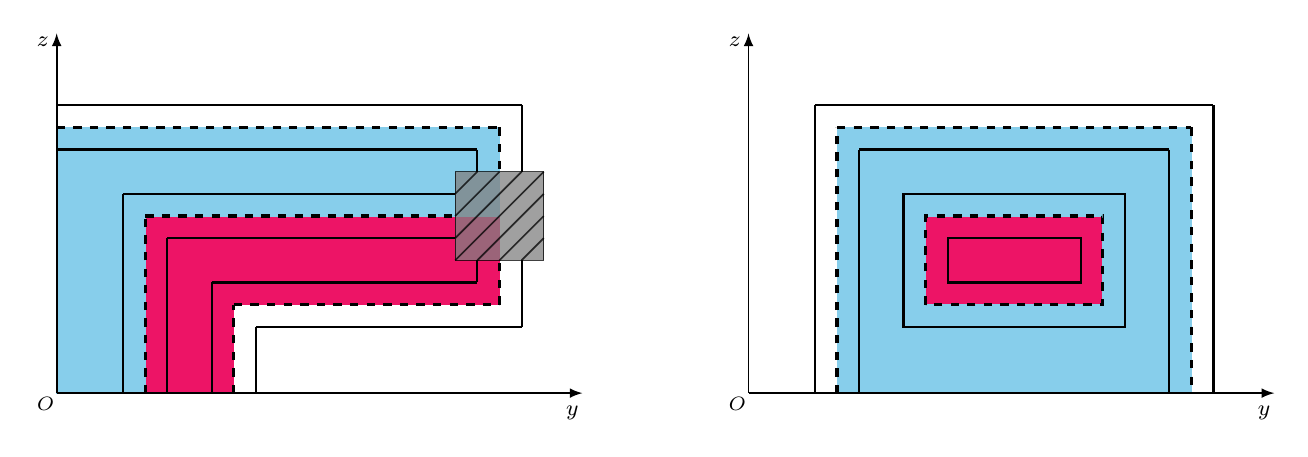
\begin{tikzpicture}[x=0.8cm, y=0.8cm, >=latex, every text node part/.style={align=center}]
    %% BEGIN left picture
    \foreach \x in {1,...,1}
        \foreach \y in {0,...,0} {
            \filldraw [fill=WildStrawberry,draw=WildStrawberry] (32pt*\x,32pt*\y) rectangle (32pt*\x+32pt, 32pt*\y+32pt);
        } 
    \foreach \x in {1,...,4}
        \foreach \y in {1,...,1} {
            \filldraw [fill=WildStrawberry,draw=WildStrawberry] (32pt*\x,32pt*\y) rectangle (32pt*\x+32pt, 32pt*\y+32pt);
        } 
    \foreach \x in {0,...,0}
        \foreach \y in {0,...,1} {
            \filldraw [fill=SkyBlue,draw=SkyBlue] (32pt*\x,32pt*\y) rectangle (32pt*\x+32pt, 32pt*\y+32pt);
        } 
    \foreach \x in {0,...,4}
        \foreach \y in {2,...,2} {
            \filldraw [fill=SkyBlue,draw=SkyBlue] (32pt*\x,32pt*\y) rectangle (32pt*\x+32pt, 32pt*\y+32pt);
        } 

    % \filldraw[draw=Gray,nearly transparent] (144pt, 48pt) rectangle (176pt, 80pt);
    \draw[draw=Black, fill=Gray, nearly opaque] (144pt, 48pt) rectangle (176pt, 80pt);
    \path[semithick,nearly opaque] (144pt,48pt) edge (176pt,80pt);
    \path[semithick,nearly opaque] (144pt,56pt) edge (168pt,80pt);
    \path[semithick,nearly opaque] (144pt,64pt) edge (160pt,80pt);
    \path[semithick,nearly opaque] (144pt,72pt) edge (152pt,80pt);
    \path[semithick,nearly opaque] (152pt,48pt) edge (176pt,72pt);
    \path[semithick,nearly opaque] (160pt,48pt) edge (176pt,64pt);
    \path[semithick,nearly opaque] (168pt,48pt) edge (176pt,56pt);

    \path[Black,very thick,dashed] (32pt, 0pt) edge (32pt, 64pt);
    \path[Black,very thick,dashed] (32pt, 64pt) edge (144pt, 64pt);
    \path[Black,thick] (24pt, 0pt) edge (24pt, 72pt);
    \path[Black,thick] (24pt, 72pt) edge (144pt, 72pt);
    \path[Black,thick] (40pt, 0pt) edge (40pt, 56pt);
    \path[Black,thick] (40pt, 56pt) edge (144pt, 56pt);
    \path[Black,very thick,dashed] (0pt, 96pt) edge (160pt, 96pt);
    \path[Black,very thick,dashed] (160pt, 96pt) edge (160pt, 80pt);
    \path[Black,thick] (0pt, 104pt) edge (168pt, 104pt);
    \path[Black,thick] (168pt, 104pt) edge (168pt, 80pt);
    \path[Black,thick] (0pt, 88pt) edge (152pt, 88pt);
    \path[Black,thick] (152pt, 88pt) edge (152pt, 80pt);
    \path[Black,very thick,dashed] (64pt, 0pt) edge (64pt, 32pt);
    \path[Black,very thick,dashed] (64pt, 32pt) edge (160pt, 32pt);
    \path[Black,very thick,dashed] (160pt, 32pt) edge (160pt, 48pt);
    \path[Black,thick] (56pt, 0pt) edge (56pt, 40pt);
    \path[Black,thick] (56pt, 40pt) edge (152pt, 40pt);
    \path[Black,thick] (152pt, 40pt) edge (152pt, 48pt);
    \path[Black,thick] (72pt, 0pt) edge (72pt, 24pt);
    \path[Black,thick] (72pt, 24pt) edge (168pt, 24pt);
    \path[Black,thick] (168pt, 24pt) edge (168pt, 48pt);

    \path[->,semithick] (0pt, 0pt) edge (0pt, 130pt);
    \path[->,semithick] (0pt, 0pt) edge (190pt, 0pt);
    \node [] () at (-4pt, -4pt) {\scriptsize $O$};
    \node [] () at (186.3pt, -7pt) {\footnotesize $y$};
    \node [] () at (-5pt, 127pt) {\footnotesize $z$};
    %% END left picture

    %% BEGIN left picture
    \foreach \x in {2,...,3}
        \foreach \y in {1,...,1} {
            \filldraw [fill=WildStrawberry,draw=WildStrawberry] (32pt*\x+250pt,32pt*\y) rectangle (32pt*\x+282pt, 32pt*\y+32pt);
        } 
    \foreach \x in {1,...,1}
        \foreach \y in {0,...,2} {
            \filldraw [fill=SkyBlue,draw=SkyBlue] (32pt*\x+250pt,32pt*\y) rectangle (32pt*\x+282pt, 32pt*\y+32pt);
        } 
    \foreach \x in {4,...,4}
        \foreach \y in {0,...,2} {
            \filldraw [fill=SkyBlue,draw=SkyBlue] (32pt*\x+250pt,32pt*\y) rectangle (32pt*\x+282pt, 32pt*\y+32pt);
        } 
    \foreach \x in {2,...,3}
        \foreach \y in {0,...,0} {
            \filldraw [fill=SkyBlue,draw=SkyBlue] (32pt*\x+250pt,32pt*\y) rectangle (32pt*\x+282pt, 32pt*\y+32pt);
        } 
    \foreach \x in {2,...,3}
        \foreach \y in {2,...,2} {
            \filldraw [fill=SkyBlue,draw=SkyBlue] (32pt*\x+250pt,32pt*\y) rectangle (32pt*\x+282pt, 32pt*\y+32pt);
        } 
    
    \draw [draw=Black,very thick,dashed] (314pt, 32pt) rectangle (378pt, 64pt);
    \path [Black,very thick,dashed] (282pt, 0pt) edge (282pt, 96pt);
    \path [Black,very thick,dashed] (282pt, 96pt) edge (410pt, 96pt);
    \path [Black,very thick,dashed] (410pt, 96pt) edge (410pt, 0pt);

    \draw [draw=Black,thick] (306pt, 24pt) rectangle (386pt, 72pt);
    \draw [draw=Black,thick] (322pt, 40pt) rectangle (370pt, 56pt);
    \path [Black,thick] (274pt, 0pt) edge (274pt, 104pt);
    \path [Black,thick] (274pt, 104pt) edge (418pt, 104pt);
    \path [Black,thick] (418pt, 104pt) edge (418pt, 0pt);
    \path [Black,thick] (290pt, 0pt) edge (290pt, 88pt);
    \path [Black,thick] (290pt, 88pt) edge (402pt, 88pt);
    \path [Black,thick] (402pt, 88pt) edge (402pt, 0pt);

    \path[->,semithick] (250pt, 0pt) edge (250pt, 130pt);
    \path[->,semithick] (250pt, 0pt) edge (440pt, 0pt);
    \node [] () at (246pt, -4pt) {\scriptsize $O$};
    \node [] () at (436.3pt, -7pt) {\footnotesize $y$};
    \node [] () at (245pt, 127pt) {\footnotesize $z$};
    %% END left picture
\end{tikzpicture}